%This is the section: Shift taker of the RTPC Operating Manual

\subsection{Shift Taker Resposibilities}
 The shift takers in the counting house have following responsibilities with regard to RTPC system:
 \begin{enumerate}
 	\item Updating the Hall B Electronic Logbook with records of system conditions (sub-section \ref{sub-sec:logbook} )
 	\item Responding to RTPC system alarms for the Hall B Alarm handler (sub-section \ref{sub-sec:alarm})
 	\item Contacting RTPC system on-call personnel (sub-section \ref{sub-sec:contact})
 	\item Monitoring the BONuS/RTPC sub-systems (sub-section \ref{sub-sec:rtpc_monitoring})
 	\begin{enumerate}[label=(\alph*)]
 		\item Monitoring the RTPC Gas system (sub-section \ref{sub-sec:gasflow})
 		\item Turning ON and OFF the HV of the RTPC detector using HV Control Interface (sub-section \ref{sub-sec:HV} )
 		\item Monitoring LV of FEUs in RTPC readout electronics (sub-section \ref{sub-sec:LV})
 		\item Monitoring the hit occupancy scalers of the system (sub-section \ref{sub-sec:monitoring})
 	\end{enumerate}
 \end{enumerate}
\subsection{Updating the Logbook}
\label{sub-sec:logbook}
The electronic logbook is set up to run on a specified terminal in the Hall B Counting House. Shift takers are responsible for keeping the records of the monitoring of RTPC sub-systems (Gas, HV, LV in RTPC Overview) and occupancy. Shift takers are also responsible for keeping an up-to-date and accurate record of any problems or issues concerning the RTPC system. For any questions regarding the logbook, its usage, or on what is considered to be a “logbook worthy” entry, consult the Leader or Run Coordinator.

Note the shift worker should follow all posted or communicated instructions about entering RTPC monitoring histograms or scaler information into the e-log. This is typically done (at least) once per run as directed on the shift checklist.

\subsection{Hall B Alarm Handler}
\label{sub-sec:alarm}

The BEAST alarm handler system running in the Counting House monitors the entire Hall B Slow Controls system. This includes the HV and low voltage (LV) systems, gas systems, torus and solenoid controls, subsystem environment controls (e.g. temperature, humidity), and pulser calibration systems (among several others), details can be seen in figure \ref{fig:alarm_screen}. The system runs on a dedicated terminal in the Counting House. One of the main responsibilities of the shift worker is to respond to alarms from this system, either by taking corrective action following guidance on alarms or by contacting the appropriate on-call personnel. Instructions and details on the alarm handler for Hall B are given in Ref. \cite{alarm-page}.

For the RTPC system there are three elements that are monitored by the alarm handler. The first is the HV system. Any time a channel trips off an alarm will sound. Trip in one channel turn off the HV to all the channels in the RTPC. These channels can be reset either through the RTPC HV control screens. These channels should be reset only after ensuring that whatever condition caused the trip (any interlocks) has been addressed. The second RTPC element monitored by the alarm handler is the gas supply to the RTPC. An overpressure or underpressure condition at any monitored point in the system will cause the HV power supply to trip off. These conditions are not expected to occur during normal operation of the RTPC gas supply. If such an alarm condition occurs, the RTPC on-call expert should be contacted to investigate and restore the system.

\begin{figure}[H]
	\centering
	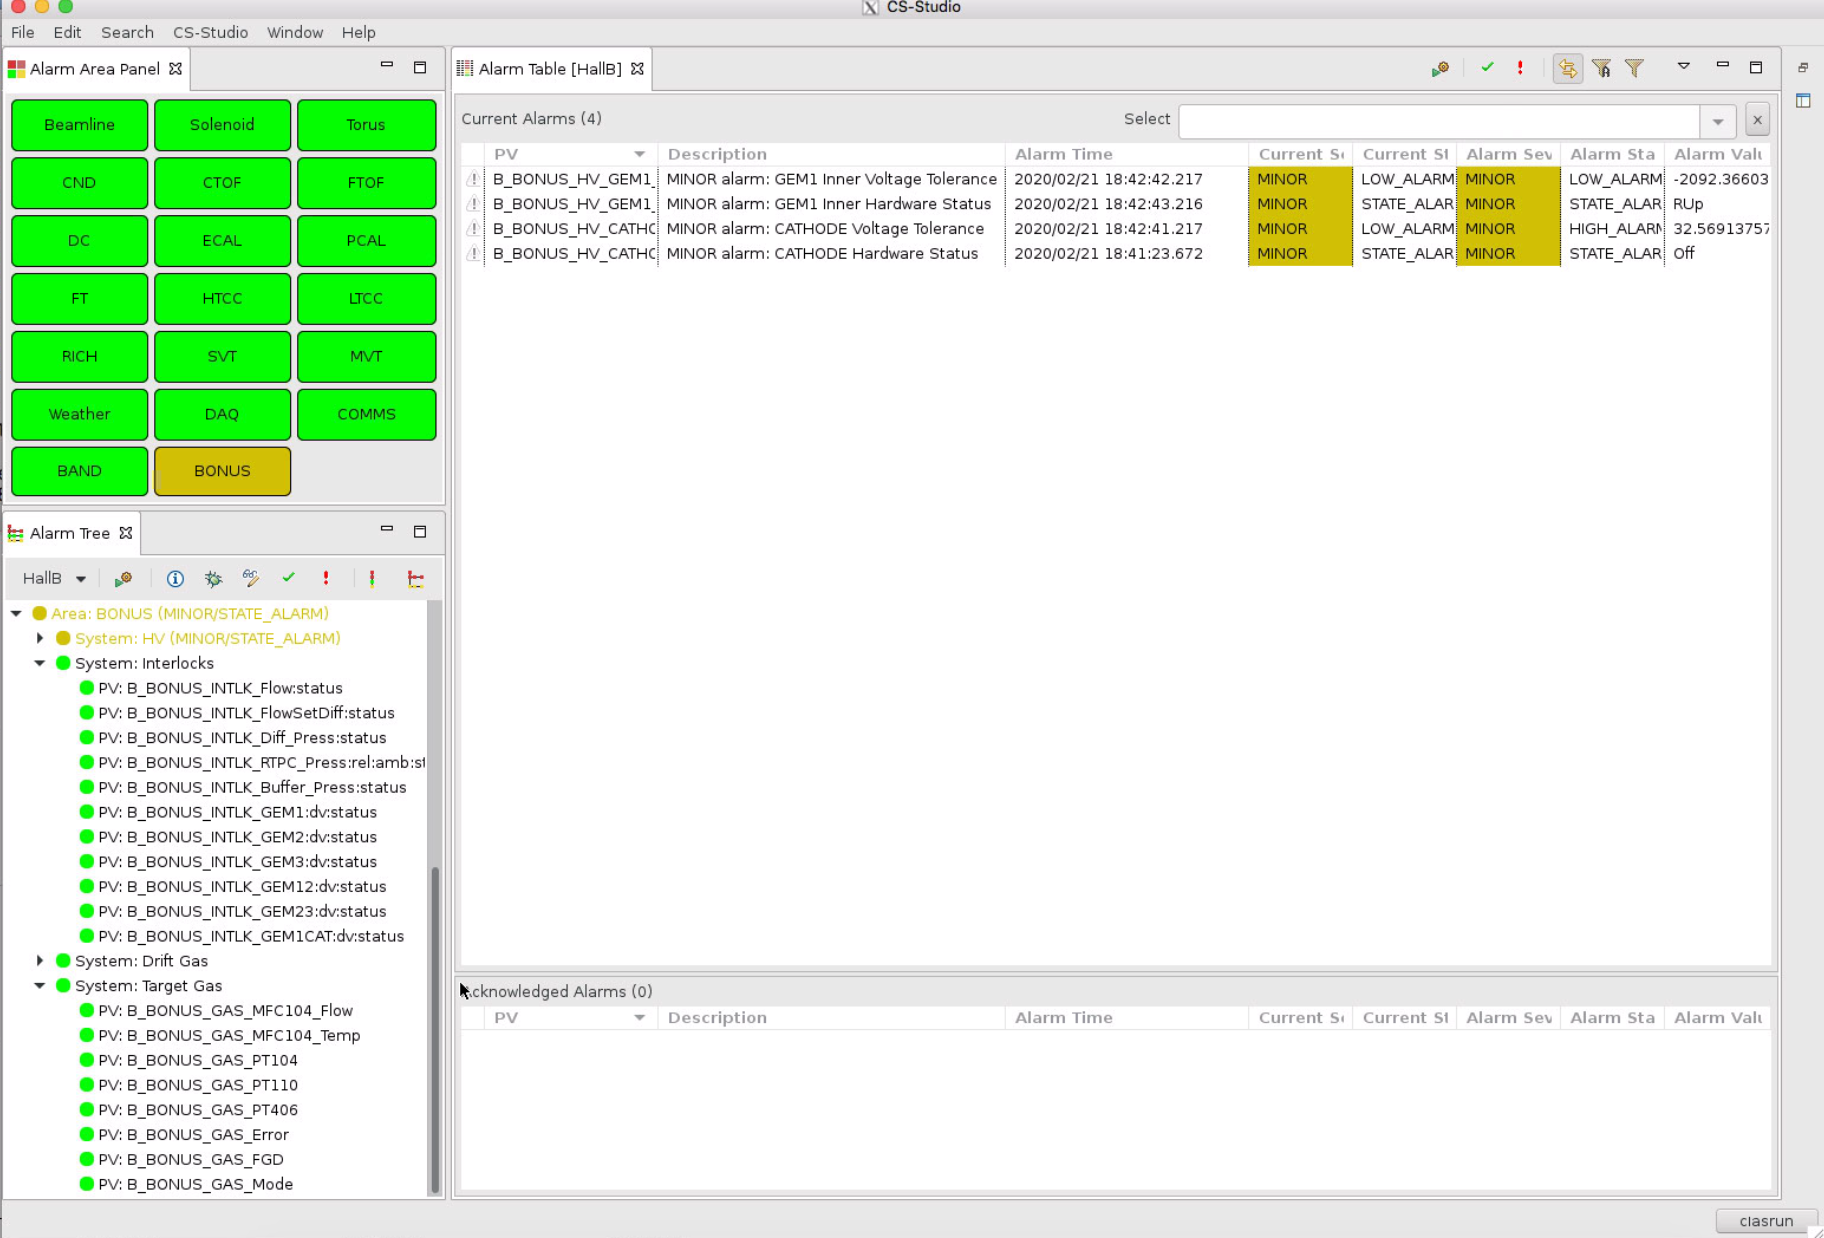
\includegraphics[width=13.5cm]{alarm_screen}
	\caption{Alarm handler in counting house}
	\label{fig:alarm_screen}
\end{figure}

There is also alarm for the BONuS target (pressurised deuterium gas $\sim$65 psig). Overpressure or underpressure of the target gas provides alarm. For the target alarm, contact the RTPC/BONuS on-call expert. RTPC expert purges the target gas daily being in counting house, so acknowledge the target alarms during purging, except it is an alarm for the `error'.
	
\subsection{Contacting the RTPC system Experts}
\label{sub-sec:contact}

As a general rule, shift takers should spend no more than 10 to 15 minutes attempting to solve any problem that arises with the RTPC system. At that point they should contact the assigned RTPC on-call expert either to get advice on how to proceed or to address the problem. The RTPC on-call phone number is {\color{red}757-329-4844}.

Only the system experts are authorized to make changes to the RTPC parameter settings, to work on the hardware or electronics, or to modify the DAQ system software. This division between shift taker and expert responsibilities is essential to maintain in order to protect and safeguard the equipment, to ensure data collection is as efficient as possible, and to minimize down time. If the shift worker has any questions regarding how to proceed when an issue arises, the shift leader should be consulted.\\

\begin{figure}[H]
	\centering
	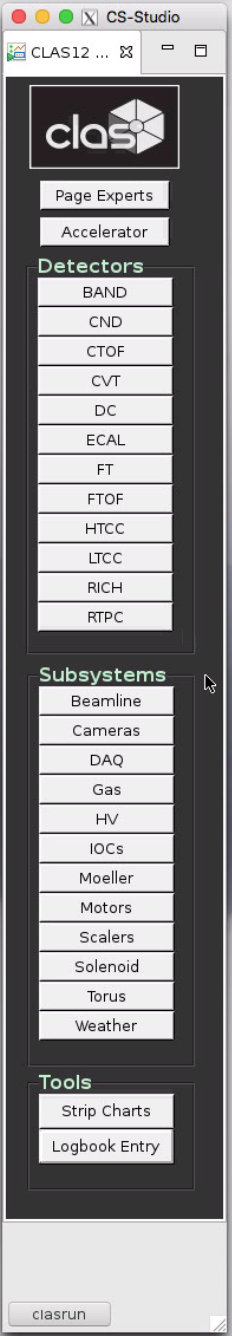
\includegraphics[height=15cm, width=3cm]{clascss}
	\qquad
	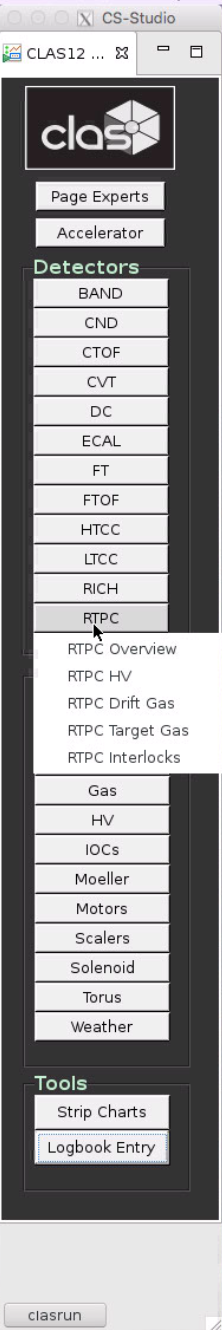
\includegraphics[height=15cm, width=3cm]{clascss1}
	\caption{CS-Studio for the slow controls of the CLAS12 (left: general, right: RTPC options)}
	\label{fig:cs-studio}
\end{figure}


\subsection{Monitoring the BONuS/RTPC sub-systems}
\label{sub-sec:rtpc_monitoring}

RTPC Overview (BONuS Overview) is under ``RTPC” of the detector sub-systems in the CLAS12 CS-Studio as shown in figure \ref{fig:cs-studio}. CS- Studio is obtained using the command ’clascss’ in the Linux terminal of counting house computers. Along with the RTPC Overview, other sub-menus (RTPC HV, RTPC Drift gas, target gas and Interlocks) are also under ``RTPC" menu. BONuS sub-system GUI are obtained either clicking these sub-menus or from clicking link in the Overview screen shown in figure \ref{fig:overview}.\\

\begin{figure}[H]
	\centering
	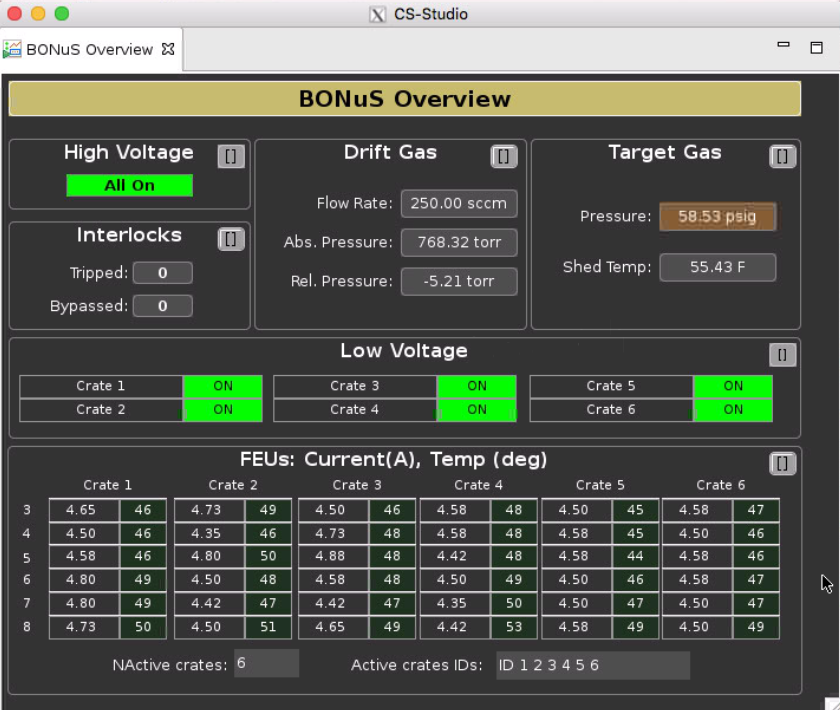
\includegraphics[height=13cm,width=13.5cm]{overview_bonus}
	\caption{BONuS/RTPC Overview GUI}
	\label{fig:overview}
\end{figure}

\subsubsection{Monitoring the BONuS12 Gas system}
\label{sub-sec:gasflow}

There are two separate gas flow lines to the RTPC detector. Helium gas is flowing in the buffer region, and pre-mixed gas [He (80\%) and CO2 (20\%)] is flowing in the drift region of the RTPC.

Clicking on the ``RTPC Gas" menu under RTPC options, we get BONuS Gas Monitoring Interface as shown in figure \ref{fig:gas_monitoring}. Flow rate of gas and the pressure inside the RTPC should be within a specified limit. If it croses the limits, alarm will be activated along with the RTPC HV interlocks. So, monitoring of this is required for the uninterrupted and better perfomance of the RTPC. 
\begin{figure}[H]
	\centering
	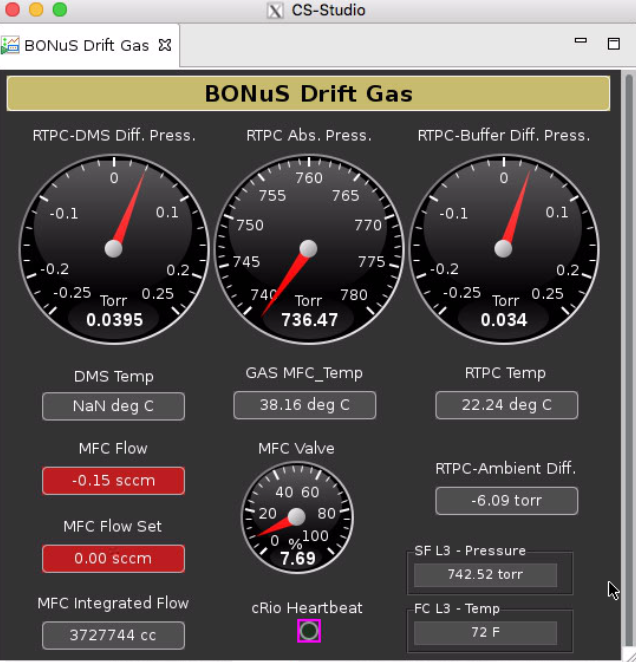
\includegraphics[scale=1]{gas_monitoring}
	\caption{RTPC Gas Monitoring Interface}
	\label{fig:gas_monitoring}
\end{figure}

\subsubsection{Monitoring and Control of the RTPC HV system}
\label{sub-sec:HV}

Novice GUI shows the status of the GEMs and cathode HV of the RTPC, but doesn't show the turn ON and OFF option for the individual channel. There are ``All ON" and ``All OFF" bottom on top (and also under menu option) to turn all channels ON/OFF. HV powering sequence is within the "All ON" bottom, so clicking it starts powering on sequence from Cathode to the GEM3 Out. It takes about 1 minutes to see the ``ramping up" status in all the channels. ``All OFF" doesn't have powering down sequence, so all the channels starts ramping down at once when ``All OFF" is clicked.

If any channel trips or kills during ramping up or down, wait until all the channels show ``OFF" status to turn them back ``ON" . If any channel shows ``kill" status, there is no need to clear it individually. Clicking ``All ON" will clear the ``kill", and start the turning on sequence from `Cathode to GEM3'. But, wait until Vmon shows $\sim$0V  in all the channels before cllicking ``All ON".

{\color{red}Note:} If ``All ON" doesn't start ramping up channels but only cleared the killed channel, please reclick the ``All ON" after about 1 minutes. Also, if you click ``All ON" before all the channels show `OFF' status, you will probably get `output failure' alarm which can be cleared with the help of an RTPC expert. Furthermore, if any interlock is active which can be seen as `Tripped' in the RTPC overview GUI (figure \ref{fig:overview}), HV can not be turned ON. To clear the interlock, help of an RTPC expert is required.
\begin{figure}[H]
	\centering
	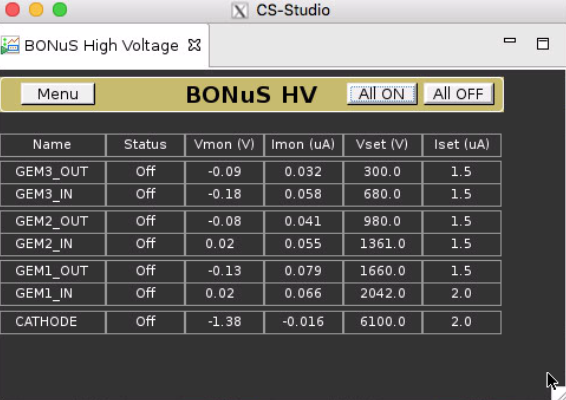
\includegraphics[height=6.5cm,width=11cm]{hv_novice}
	\caption{RTPC HV control Interface for Novice}
	\label{fig:hv_novice1}
\end{figure}

\subsubsection{Monitoring the RTPC LV system}
\label{sub-sec:LV}

Low voltage is applied to the Front End electronics of the RTPC data aqcuisition. RTPC and FMT share the common power supply to the Front End Units (FEUs). Low Voltage (LV) power supply is monitored from the RTPC Overview GUI as shown in figure \ref{fig:overview}. When there is an issue with LV, both RTPC and FMT are affected. Low voltage power cycle could be done safely by experts, as it can activate the interlock for both RTPC and FMT HV with some delay. 

\subsubsection{Monitoring the Hit Occupancy}
\label{sub-sec:monitoring}
Hit occupancy of the RTPC detector looks like as shown in figure \ref{fig:occupancy}. Comparision of the monitoring plot with the attached picture is required. If the monitoring looks completely different than the attached one, please inform the Run-cordinator or the RTPC expert on call.
\begin{figure}[H]
	\centering
	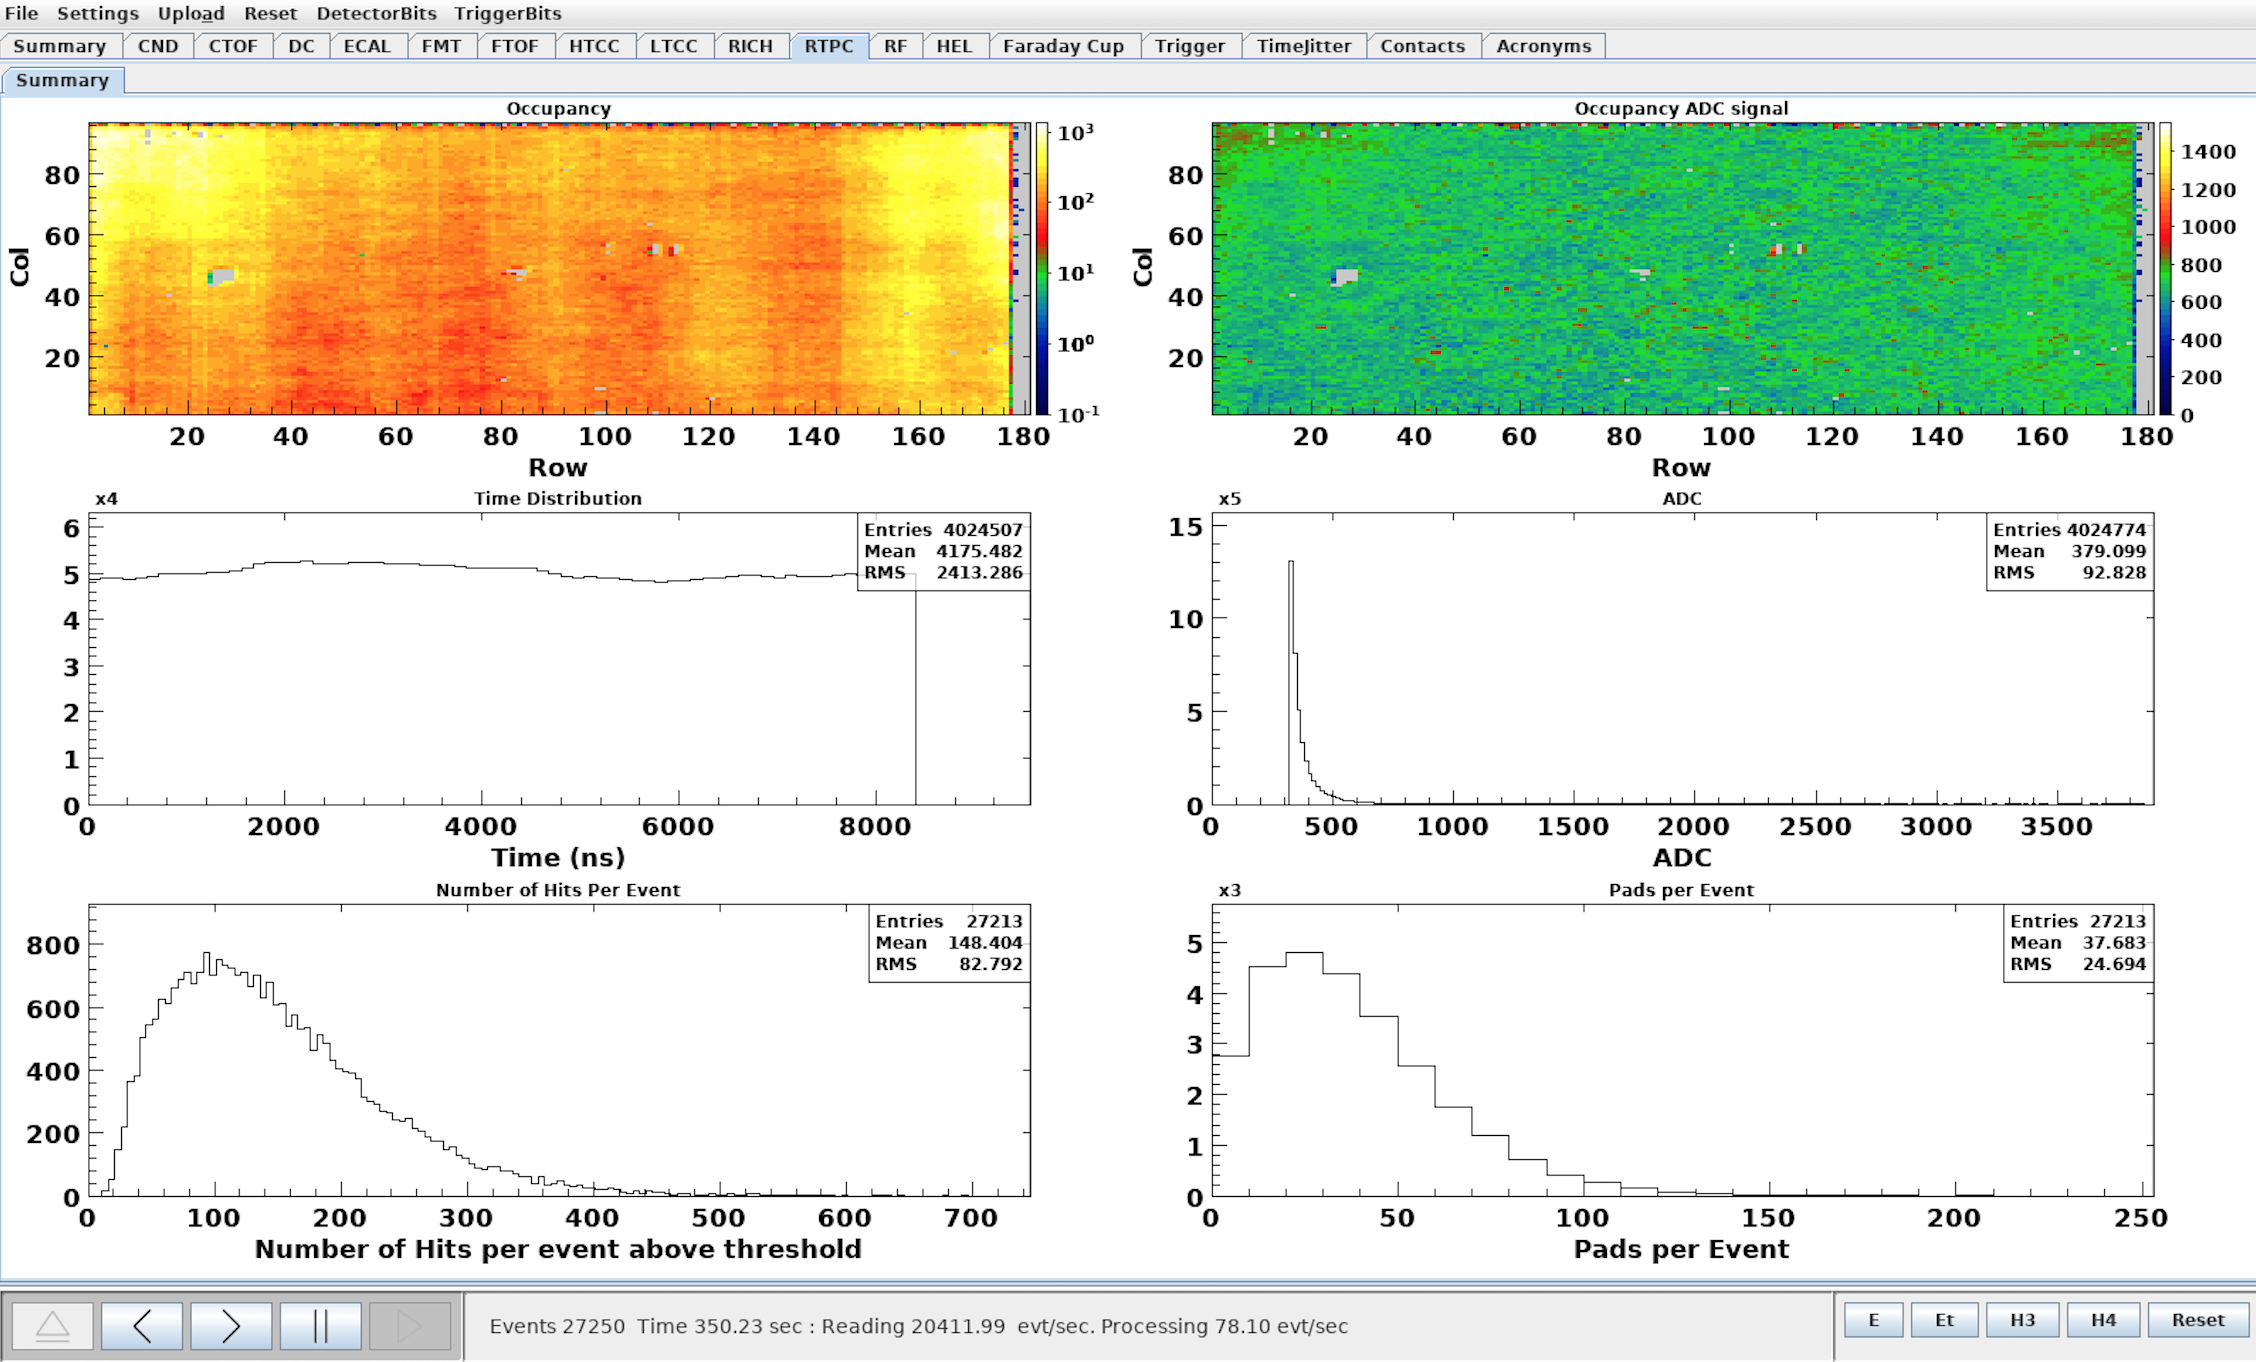
\includegraphics[height=10cm,width=13.5cm]{occupancy.png}
	\caption{Occupancy monitoring of the RTPC}
	\label{fig:occupancy}
\end{figure}